\documentclass{article}

\usepackage{pgfplots}
\pgfplotsset{compat=1.16}

\begin{document}
    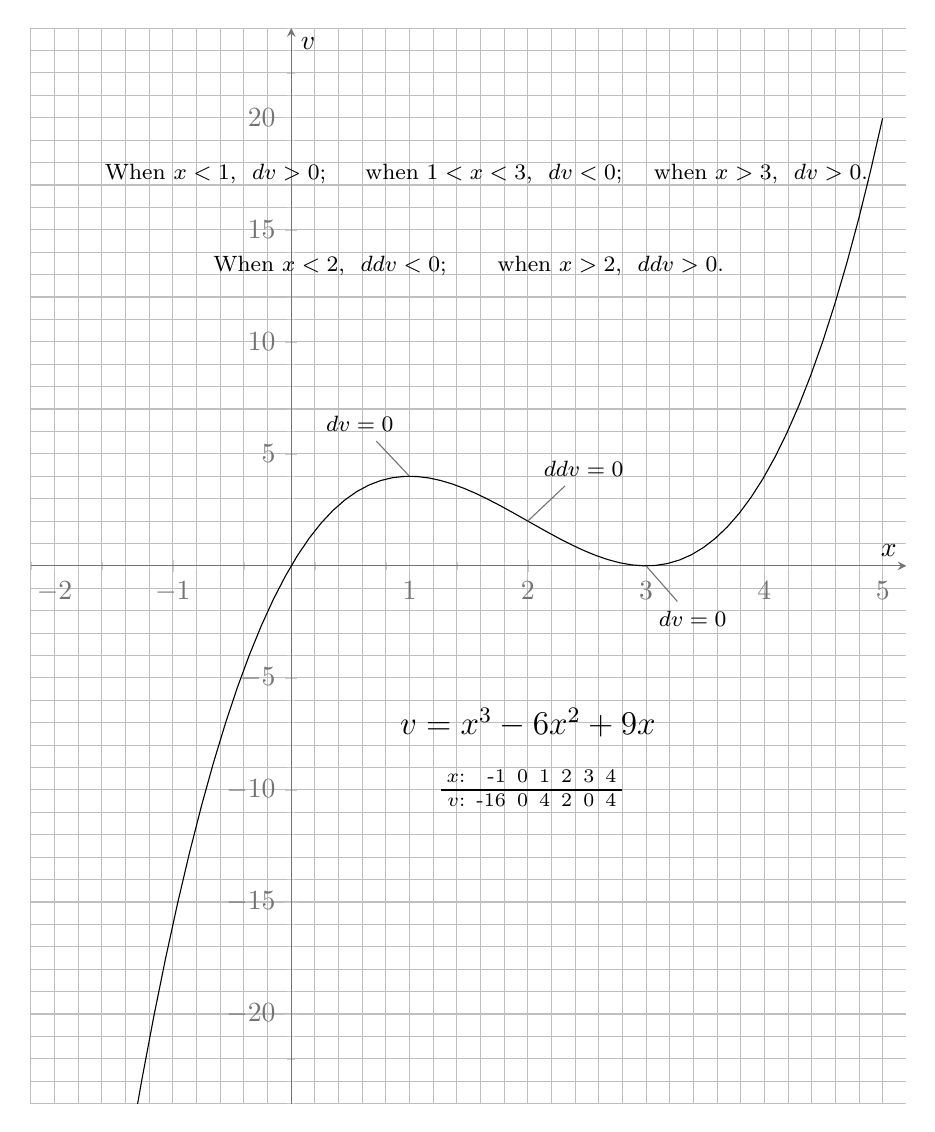
\begin{tikzpicture}
    \tikzset{%
      % every pin/.style={fill=gray!10, rectangle, rounded corners=3pt}
      every pin edge/.style={black!55}    
    }  
    \begin{axis}[axis line style={black!55},
      axis lines=middle,
      %label style={black},%!45}, how dark the xlabel etc are
      xlabel={$x$}, ylabel=$v$,
      % grid style={black!5},
      % grid style={black!20},
      xmajorgrids=true, ymajorgrids=true,
      xminorgrids=true, yminorgrids=true,
      % tick label style={black!40},
      tick label style={black!55},
      tick style={gray!40},
      %tick style={black!60},
      minor x tick num=4, minor y tick num=4,
      ymin=-24, ymax=24,
      xmin=-2.2, xmax=5.2,
      width=5in, height=6in, samples=100, ]
      \node[] at (1.65,17.5)
      {\footnotesize When $x<1,\hspace{0.5em} dv>0;$ \hspace{1em}
        when $1<x<3, \hspace{0.5em} dv<0;$\hspace{1em}
        when $x>3,\hspace{0.5em} dv>0.$};
      \node[] at (1.5,13.4) {\footnotesize When $x<2,
        \hspace{0.5em} ddv<0;$ \hspace{1.5em}
        when $x>2, \hspace{0.5em} ddv>0.$};
      \addplot [ black,] {x^3 - 6*x^2 + 9*x};
      \node[coordinate, pin=100:{\footnotesize$dv=0$}] at (1,4) {};
      \node[coordinate, pin=275:{\footnotesize$dv=0$}] at (3,0) {};
      \node[coordinate, pin=80:{\footnotesize$ddv=0$}] at (2,2) {};
      \node[] at (2,-7) {\large $v=x^3 -6x^2+ 9x$};
      \node[] at (2,-10) {\scriptsize
        \setlength{\tabcolsep}{2pt}
        \begin{tabular}{rrrrrrr}
          $x$:&-1&0&1&2&3&4\\ \hline
          $v$:&-16&0&4&2&0&4
        \end{tabular}};
    \end{axis}
  \end{tikzpicture}

\end{document}

    \begin{tikzpicture}
    \begin{axis}[axis line style={black!55},
      axis lines=middle,
      axis label style={black!55},
      xlabel={$x$}, ylabel=$v$,
      % grid style={black!5},
      %grid style={black!20},
      xmajorgrids=true, ymajorgrids=true,
      xminorgrids=true, yminorgrids=true,
      % tick label style={black!40},
      tick label style={black!55},
      %tick style={gray!40},
      tick style={black!20},
      minor x tick num=4, minor y tick num=4,
      label style={black!45},
      ymin=-20, ymax=25,
      xmin=-2, xmax=5,
      width=5in, height=6in, samples=100, ]
      \node[] at (1.65,17.5)
      {\footnotesize When $x<1,\hspace{0.5em} dv>0;$ \hspace{1em}
        when $1<x<3, \hspace{0.5em} dv<0;$\hspace{1em}
        when $x>3,\hspace{0.5em} dv>0.$};
      \node[] at (1.5,13.4) {\footnotesize When $x<2,
        \hspace{0.5em} ddv<0;$ \hspace{1.5em}
        when $x>2, \hspace{0.5em} ddv>0.$};
      \addplot [ black,] {x^3 - 6*x^2 + 9*x};
      \node[coordinate, pin=100:{\footnotesize$dv=0$}] at (1,4) {};
      \node[coordinate, pin=275:{\footnotesize$dv=0$}] at (3,0) {};
      \node[coordinate, pin=80:{\footnotesize$ddv=0$}] at (2,2) {};
      \node[] at (2,-7) {\large $v=x^3 -6x^2+ 9x$};
      \node[] at (2,-10) {\scriptsize
        \setlength{\tabcolsep}{2pt}
        \begin{tabular}{rrrrrrr}
          $x$:&-1&0&1&2&3&4\\ \hline
          $v$:&-16&0&4&2&0&4
        \end{tabular}};
    \end{axis}
  \end{tikzpicture}

%%% Local Variables:
%%% mode: latex
%%% TeX-master: t
%%% End:
